%%%%%%%%%%%%%%%%%%%%%%%%%%%%%%%%%%%%%%%%%
% Short Sectioned Assignment LaTeX Template Version 1.0 (5/5/12)
% This template has been downloaded from: http://www.LaTeXTemplates.com
% Original author:  Frits Wenneker (http://www.howtotex.com)
% License: CC BY-NC-SA 3.0 (http://creativecommons.org/licenses/by-nc-sa/3.0/)
%%%%%%%%%%%%%%%%%%%%%%%%%%%%%%%%%%%%%%%%%

%----------------------------------------------------------------------------------------
%	PACKAGES AND OTHER DOCUMENT CONFIGURATIONS
%----------------------------------------------------------------------------------------

\documentclass[paper=a4, fontsize=11pt]{scrartcl} % A4 paper and 11pt font size

% ---- Entrada y salida de texto -----

\usepackage[T1]{fontenc} % Use 8-bit encoding that has 256 glyphs
\usepackage[utf8]{inputenc}
\usepackage{hyperref}
%\usepackage{fourier} % Use the Adobe Utopia font for the document - comment this line to return to the LaTeX default

% ---- Idioma --------

\usepackage[spanish, es-tabla]{babel} % Selecciona el español para palabras introducidas automáticamente, p.ej. "septiembre" en la fecha y especifica que se use la palabra Tabla en vez de Cuadro

% ---- Otros paquetes ----

\usepackage{url} % ,href} %para incluir URLs e hipervínculos dentro del texto (aunque hay que instalar href)
\usepackage{amsmath,amsfonts,amsthm} % Math packages
%\usepackage{graphics,graphicx, floatrow} %para incluir imágenes y notas en las imágenes
\usepackage{graphics,graphicx, float} %para incluir imágenes y colocarlas

% Para hacer tablas comlejas
%\usepackage{multirow}
%\usepackage{threeparttable}

%\usepackage{sectsty} % Allows customizing section commands
%\allsectionsfont{\centering \normalfont\scshape} % Make all sections centered, the default font and small caps

\usepackage{fancyhdr} % Custom headers and footers
\pagestyle{fancyplain} % Makes all pages in the document conform to the custom headers and footers
\fancyhead{} % No page header - if you want one, create it in the same way as the footers below
\fancyfoot[L]{} % Empty left footer
\fancyfoot[C]{} % Empty center footer
\fancyfoot[R]{\thepage} % Page numbering for right footer
\renewcommand{\headrulewidth}{0pt} % Remove header underlines
\renewcommand{\footrulewidth}{0pt} % Remove footer underlines
\setlength{\headheight}{13.6pt} % Customize the height of the header

\numberwithin{equation}{section} % Number equations within sections (i.e. 1.1, 1.2, 2.1, 2.2 instead of 1, 2, 3, 4)
\numberwithin{figure}{section} % Number figures within sections (i.e. 1.1, 1.2, 2.1, 2.2 instead of 1, 2, 3, 4)
\numberwithin{table}{section} % Number tables within sections (i.e. 1.1, 1.2, 2.1, 2.2 instead of 1, 2, 3, 4)

\setlength\parindent{0pt} % Removes all indentation from paragraphs - comment this line for an assignment with lots of text

\newcommand{\horrule}[1]{\rule{\linewidth}{#1}} % Create horizontal rule command with 1 argument of height


%----------------------------------------------------------------------------------------
%	TÍTULO Y DATOS DEL ALUMNO
%----------------------------------------------------------------------------------------

\title{	
\normalfont \normalsize 
\textsc{\textbf{Ingeniería de Servidores (2016-2017)} \\ Grado en Ingeniería Informática \\ Universidad de Granada} \\ [25pt] % Your university, school and/or department name(s)
\horrule{0.5pt} \\[0.4cm] % Thin top horizontal rule
\huge Memoria Práctica 3 \\ % The assignment title
\horrule{2pt} \\[0.5cm] % Thick bottom horizontal rule
}

\author{Sergio Samaniego Martínez} % Nombre y apellidos

\date{\normalsize\today} % Incluye la fecha actual

%----------------------------------------------------------------------------------------
% DOCUMENTO
%----------------------------------------------------------------------------------------

\begin{document}

\maketitle % Muestra el Título

\newpage %inserta un salto de página

\tableofcontents % para generar el índice de contenidos

\newpage

\section{Cuestión 1}

\subsection{\Large¿Qué archivo le permite ver qué programas se han instalado con el gestor de paquetes? }

El archivo que nos permite ver qué programas se han instalado con el gestor de paquetes es el archivo de registro de dpkg, el cual se encuentra en /var/log.
El archivo de registro es dpkg.log y tendrá las últimas acciones hechas con el gestor de paquetes. \cite{dpkg}

\begin{figure}[H] %con el [H] le obligamos a situar aquí la figura
	\centering
	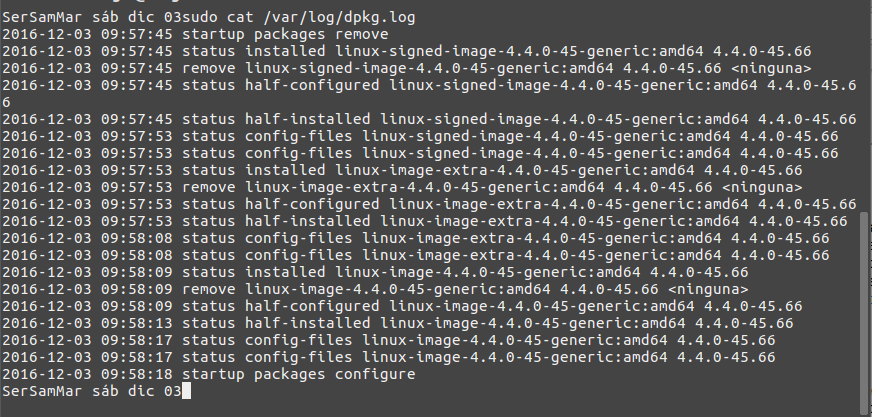
\includegraphics[scale=0.5]{imagenes/dpkg-log.png}  %el parámetro scale permite agrandar o achicar la imagen. En el nombre de archivo puede especificar directorios
	\caption{Muestra del arvhivo dpkg.log}
\end{figure}


\subsection{\Large ¿Qué significan las terminaciones .1.gz o .2.gz de los archivos en ese directorio?}

Las terminaciones de .1.gz o .2.gz son anteriores archivos de registro los cuales han sido comprimidos por el demonio cron.daily.
Este hace una rotación que se encarga de comprimir los archivos añadiéndoles la extensión .1.gz, .2.gz, etc volviendo a crear un nuevo archivo vacío.
\cite{1-gz}

\section{Cuestión 2}

\subsection{\Large ¿qué archivo ha de modificar para programar una tarea? Escriba la línea necesaria para ejecutar una vez al día una copia del directorio ~/codigo a ~/seguridad/ \$fecha donde \$fecha es la fecha actual (puede usar el comando date).}

Para programar una tarea debemos modificar el archivo crontab que se encuentra dentro del directorio /etc.
Ya dentro del archivo se le pasa la frecuencia con la que se quiere programar la tarea y el comando a ejecutar, en nuestro caso el script que ejecutará.\cite{cron} \cite{crontab}

\begin{figure}[H] %con el [H] le obligamos a situar aquí la figura
	\centering
	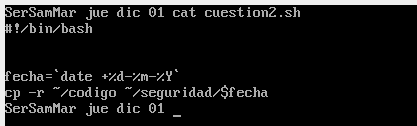
\includegraphics[scale=0.5]{imagenes/script-cron.png}  %el parámetro scale permite agrandar o achicar la imagen. En el nombre de archivo puede especificar directorios
	\caption{Script que se ejecuta en crontab diariamente}
\end{figure}

Con ese script lo que hacemos es copiar los archivos que hay en el directorio ~/codigo en el directorio ~/seguridad/fecha el cual diariamente irá cambiando ya que cada directorio creado tendrá la fecha del día que se ha hecho la copia.

Por último editamos el archivo crontab.
\begin{figure}[H] %con el [H] le obligamos a situar aquí la figura
	\centering
	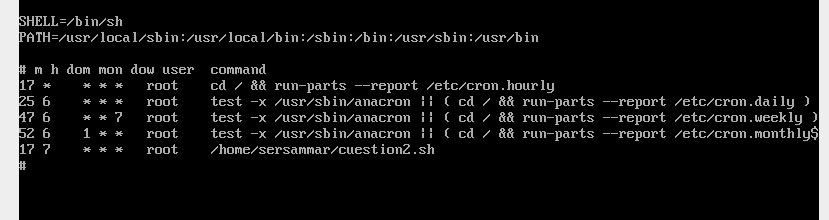
\includegraphics[scale=0.5]{imagenes/crontab.png}  %el parámetro scale permite agrandar o achicar la imagen. En el nombre de archivo puede especificar directorios
	\caption{Muestra del contenido de crontab}
\end{figure}

Como se muestra en la figura, hemos añadido la última línea para que ejecute el script mostrado anteriormente todos los días a las 7:17

Y por último reiniciar el servicio para que los cambios surjan efecto.

\section{Cuestión 3}

\subsection{\Large Pruebe a ejecutar el comando, conectar un dispositivo USB y vuelva a ejecutar el comando. Copie y pegue la salida del comando. (considere usar dmesg | tail). Comente qué observa en la información mostrada.}

Lo que he hecho ha sido ejecutar el comando dmesg sin ningún dispositivo conectado y lo he guardado en el archivo antes.
Después he conectado el dispositivo y he vuelto a ejecutar el comando guardándolo en el archivo después.

Por último muestro por pantalla la diferencia entre los dos archivos, la cual vemos que es debido a la conexión de un dispositivo USB, en concreto mi smartphone de marca Huawei como se ve en la figura.

\begin{figure}[H] %con el [H] le obligamos a situar aquí la figura
	\centering
	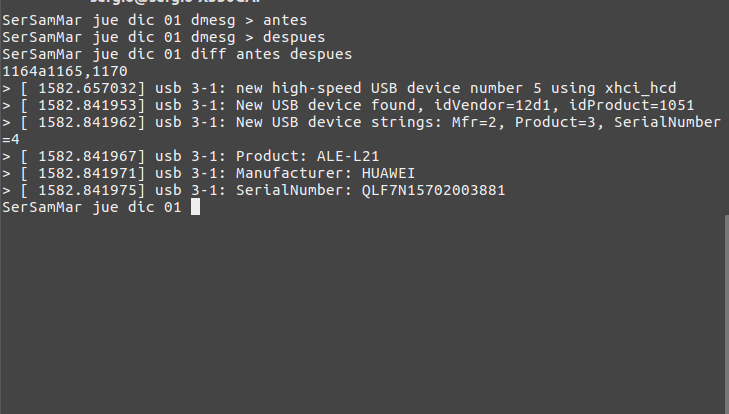
\includegraphics[scale=0.5]{imagenes/dmesg.png}  %el parámetro scale permite agrandar o achicar la imagen. En el nombre de archivo puede especificar directorios
	\caption{Muestra del contenido de crontab}
\end{figure}

\section{Cuestión 4}
\subsection{\Large Ejecute el monitor de “System Performance” y muestre el resultado. Incluya capturas de pantalla comentando la información que aparece.}

\begin{figure}[H] %con el [H] le obligamos a situar aquí la figura
	\centering
	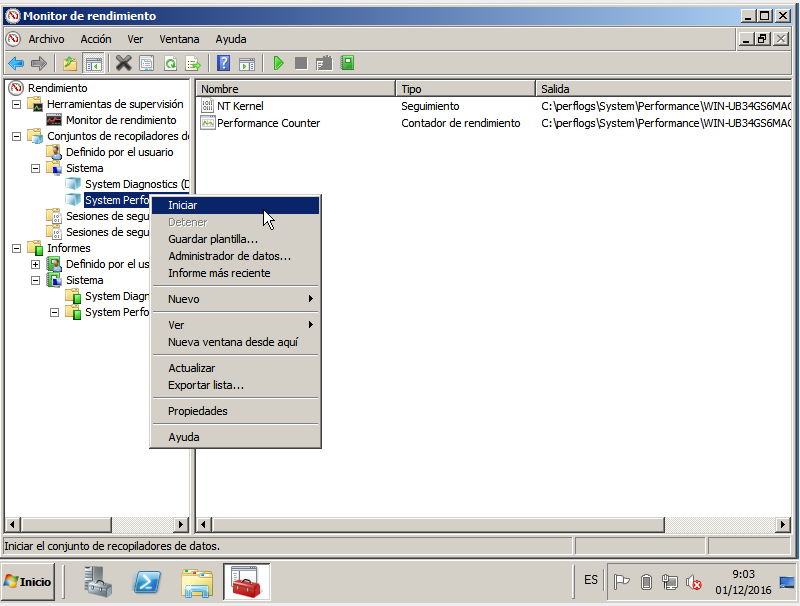
\includegraphics[scale=0.5]{imagenes/iniciar-perfmon.png}  %el parámetro scale permite agrandar o achicar la imagen. En el nombre de archivo puede especificar directorios
	\caption{Inicio del System Performance}
\end{figure}

Primero hemos ejecutado el "System Performance" sin nada abierto, por lo que sabemos que el uso de CPU del sistema va a ser muy bajo.

\begin{figure}[H] %con el [H] le obligamos a situar aquí la figura
	\centering
	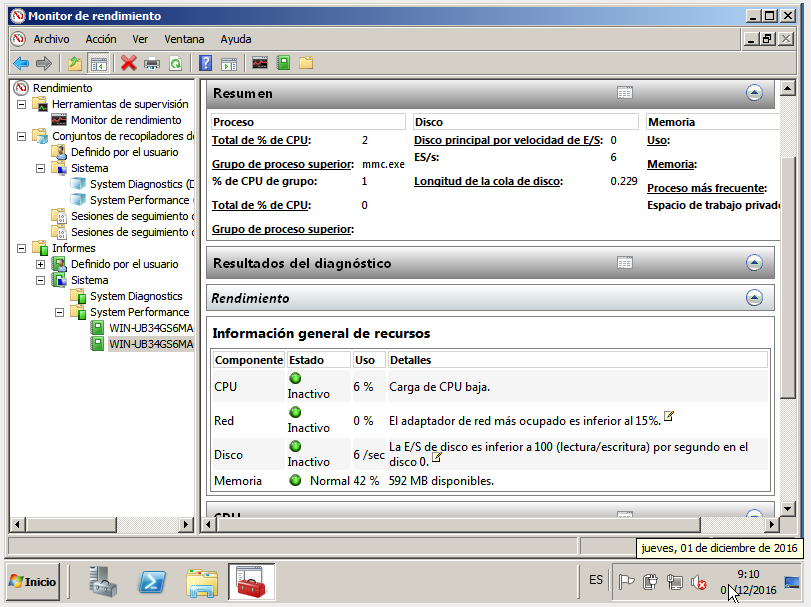
\includegraphics[scale=0.5]{imagenes/prog-cerrados.png}  %el parámetro scale permite agrandar o achicar la imagen. En el nombre de archivo puede especificar directorios
	\caption{Contenido del informe del sistema con todos los programas cerrados}
\end{figure}

Ahora para hacer una pequeña comparación hemos abierto muchas ventanas de Internet Explorer, así como otras cuantas del bloc de notas.

\begin{figure}[H] %con el [H] le obligamos a situar aquí la figura
	\centering
	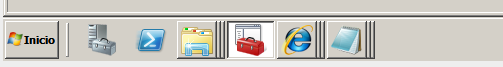
\includegraphics[scale=0.5]{imagenes/muchas-ventanas.png}  %el parámetro scale permite agrandar o achicar la imagen. En el nombre de archivo puede especificar directorios
	\caption{Ventanas abiertas para hacer el System Performance}
\end{figure}

Una vez abierto todo esto, vamos a ejecutar de nuevo el "System Performance" y a analizar los resultados.

\begin{figure}[H] %con el [H] le obligamos a situar aquí la figura
	\centering
	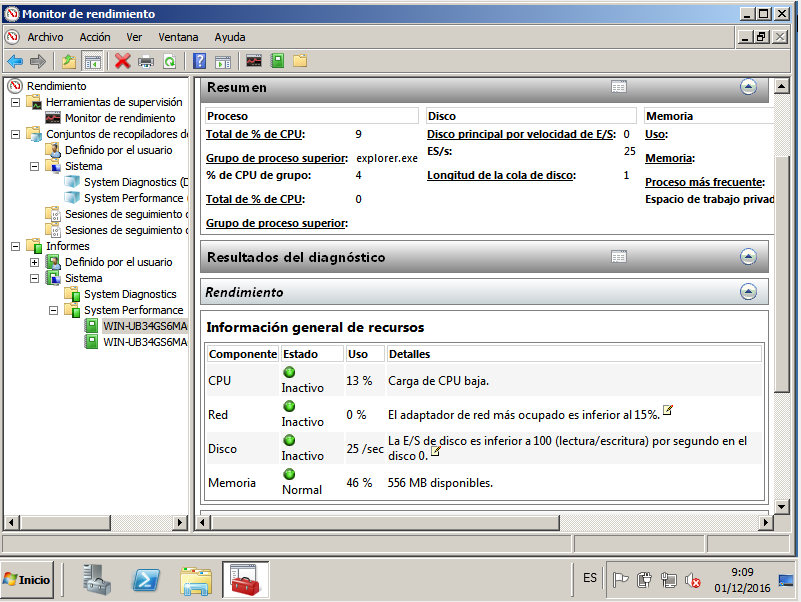
\includegraphics[scale=0.5]{imagenes/prog-abiertos.png}  %el parámetro scale permite agrandar o achicar la imagen. En el nombre de archivo puede especificar directorios
	\caption{Muestra del contenido de crontab}
\end{figure}

Como podemos ver, el porcentaje de uso del CPU aumenta con respecto al primer informe sin nada abierto, esto es normal ya que tenemos más programas abiertos, así como el uso del disco y la memoria usada.
Aún así, este informe general del sistema nos muestra que la carga de éste sistema está siendo baja, cosa que es totalmente lógica ya que no tenemos ningún programa pesado que nos esté consumiendo recursos.


\section{Cuestión 5}
\subsection{\Large Cree un recopilador de datos definido por el usuario (modo avanzado) que incluya tanto el contador de rendimiento como los datos de seguimiento:\\Todos los referentes al procesador, al proceso y al servicio web.\\Intervalo de muestra 15 segundos.\\Almacene el resultado en el directorio Escritorio/logs.\\Incluya las capturas de pantalla de cada paso.}

Para crear un recopilador de datos que hayamos definido nosotros tendremos que crearlo, para ello pinchamos con el botón derecho Nuevo->Conjunto de recopilador de datos.

\begin{figure}[H] %con el [H] le obligamos a situar aquí la figura
	\centering
	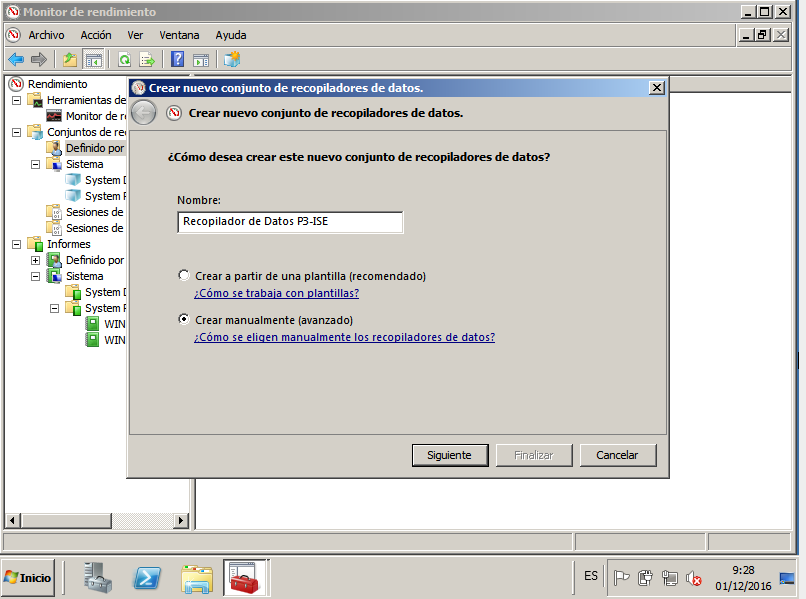
\includegraphics[scale=0.5]{imagenes/CD-1.png}  %el parámetro scale permite agrandar o achicar la imagen. En el nombre de archivo puede especificar directorios
	\caption{Define el nombre del recopilador de datos}
\end{figure}

Hecho esto daremos a Siguiente, y nos pedirá los datos que deseamos incluir.

\begin{figure}[H] %con el [H] le obligamos a situar aquí la figura
	\centering
	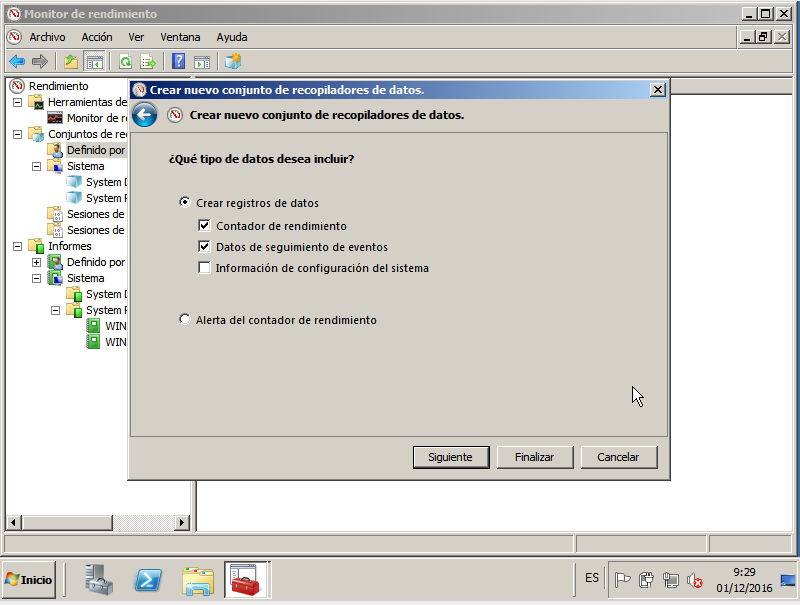
\includegraphics[scale=0.5]{imagenes/CD-2.png}  %el parámetro scale permite agrandar o achicar la imagen. En el nombre de archivo puede especificar directorios
	\caption{Incluir contador de rendimiento y datos de seguimiento}
\end{figure}

El paso siguiente será añadir los contadores que queremos, que en nuestro caso son los contadores del procesador, proceso y servicio web.

\begin{figure}[H] %con el [H] le obligamos a situar aquí la figura
	\centering
	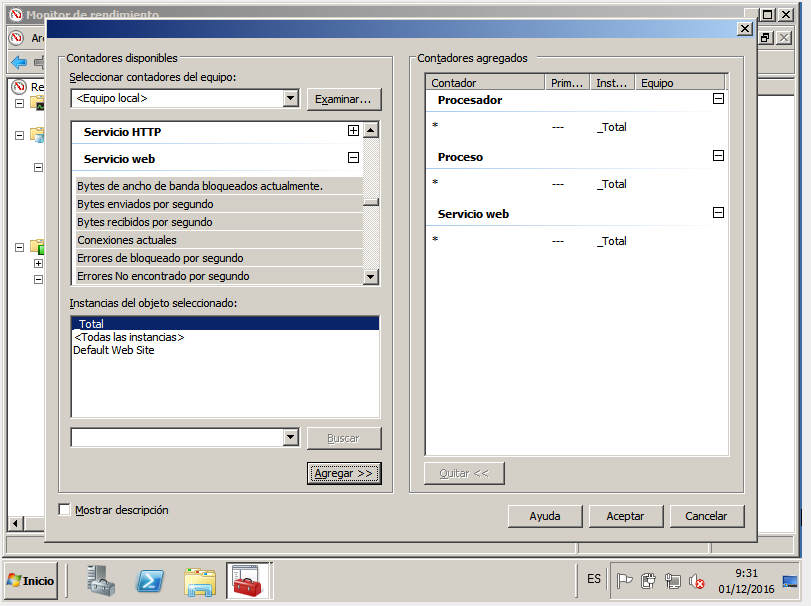
\includegraphics[scale=0.5]{imagenes/CD-3.png}  %el parámetro scale permite agrandar o achicar la imagen. En el nombre de archivo puede especificar directorios
	\caption{Añadiendo los contadores}
\end{figure}

\begin{figure}[H] %con el [H] le obligamos a situar aquí la figura
	\centering
	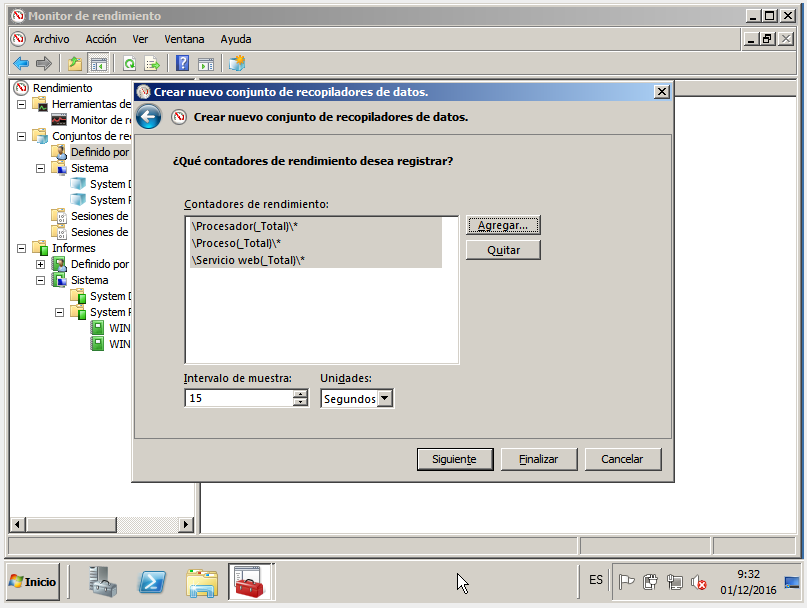
\includegraphics[scale=0.5]{imagenes/CD-4.png}  %el parámetro scale permite agrandar o achicar la imagen. En el nombre de archivo puede especificar directorios
	\caption{Definiendo el intervalo de muestreo}
\end{figure}

Damos a siguiente y añadimos los proveedores de sequimiento que deseamos.

\begin{figure}[H] %con el [H] le obligamos a situar aquí la figura
	\centering
	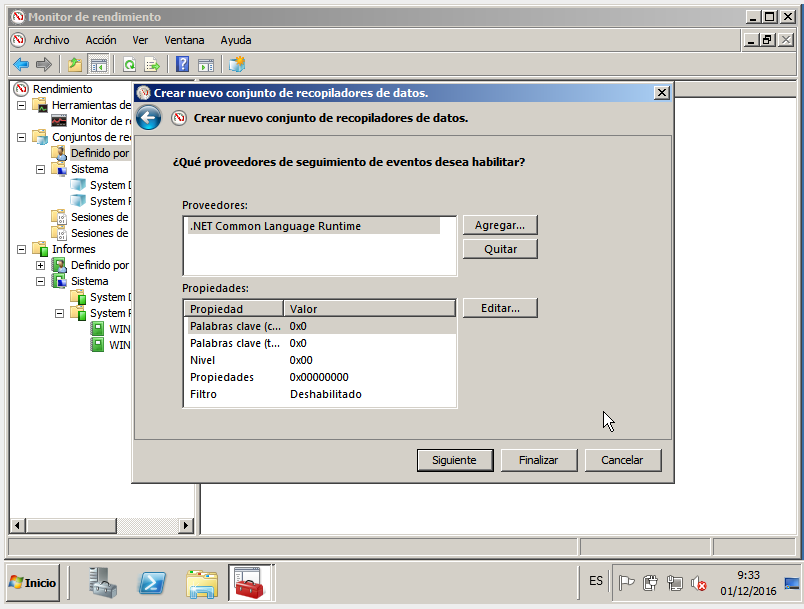
\includegraphics[scale=0.5]{imagenes/CD-5.png}  %el parámetro scale permite agrandar o achicar la imagen. En el nombre de archivo puede especificar directorios
	\caption{Proveedor añadido}
\end{figure}

Paso siguiente es indicarle dónde vamos a guardar los datos, en nuestro caso en Desktop/logs

\begin{figure}[H] %con el [H] le obligamos a situar aquí la figura
	\centering
	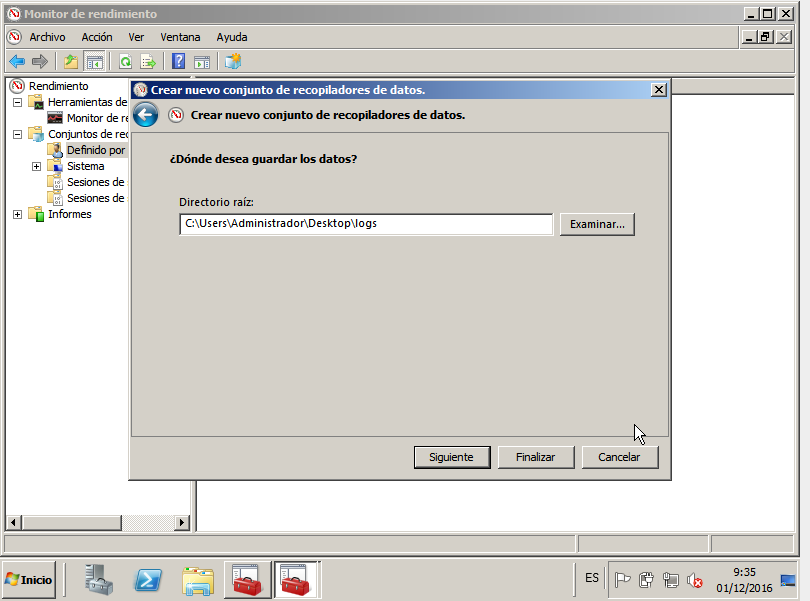
\includegraphics[scale=0.5]{imagenes/CD-6.png}  %el parámetro scale permite agrandar o achicar la imagen. En el nombre de archivo puede especificar directorios
	\caption{Ruta donde guardaremos los datos}
\end{figure}

Ahora ya tenemos creado nuestro propio recopilador de datos. Para mostrarlo lo iniciaremos y veremos los datos recopilados.

\begin{figure}[H] %con el [H] le obligamos a situar aquí la figura
	\centering
	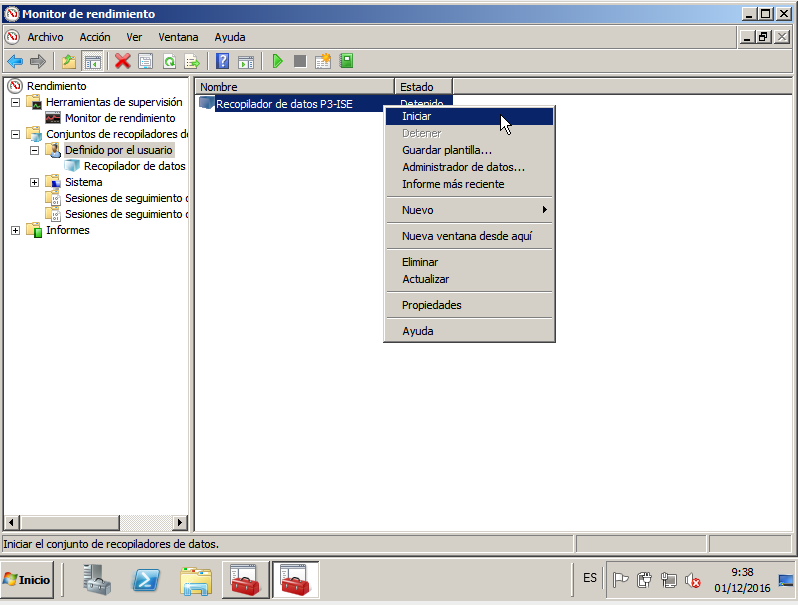
\includegraphics[scale=0.5]{imagenes/CD-8.png}  %el parámetro scale permite agrandar o achicar la imagen. En el nombre de archivo puede especificar directorios
	\caption{Iniciamos nuestro recopilador de datos}
\end{figure}

Una vez iniciado, nos vamos a la carpeta que indicamos anteriormente, en nuestro caso /Desktop/logs donde tendremos nuestro archivo de monitor.

\begin{figure}[H] %con el [H] le obligamos a situar aquí la figura
	\centering
	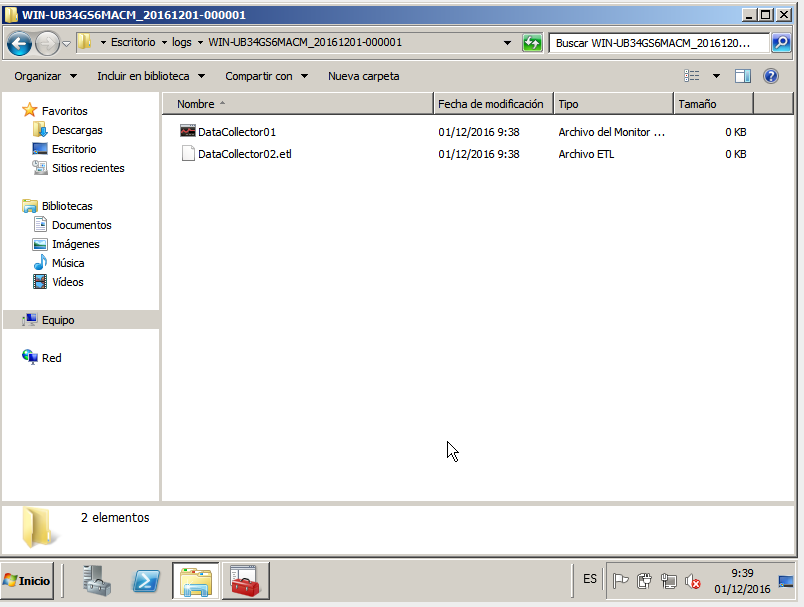
\includegraphics[scale=0.5]{imagenes/CD-9.png}  %el parámetro scale permite agrandar o achicar la imagen. En el nombre de archivo puede especificar directorios
	\caption{Archivos de /Desktop/logs}
\end{figure}

Por último, abrimos el archivo y nos mostrará la ejecución del monitor con los datos que se le indicó.

\begin{figure}[H] %con el [H] le obligamos a situar aquí la figura
	\centering
	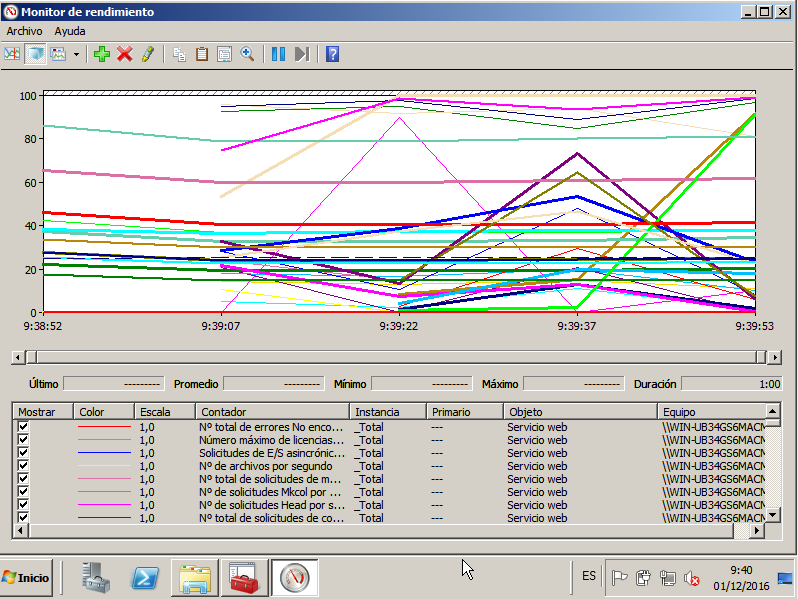
\includegraphics[scale=0.5]{imagenes/CD-10.png}  %el parámetro scale permite agrandar o achicar la imagen. En el nombre de archivo puede especificar directorios
	\caption{Archivo de monitor.}
\end{figure}

\section{Cuestión 6}

\subsection{\Large Visite la web del proyecto y acceda a la demo que proporcionan (http://demo.munin-monitoring.org/) donde se muestra cómo monitorizan un servidor. Monitorice varios parámetros y haga capturas de pantalla de lo que está mostrando comentando qué observa.}

El primer parámetro que vamos a monitorizar es el uso de red por día.

\begin{figure}[H] %con el [H] le obligamos a situar aquí la figura
	\centering
	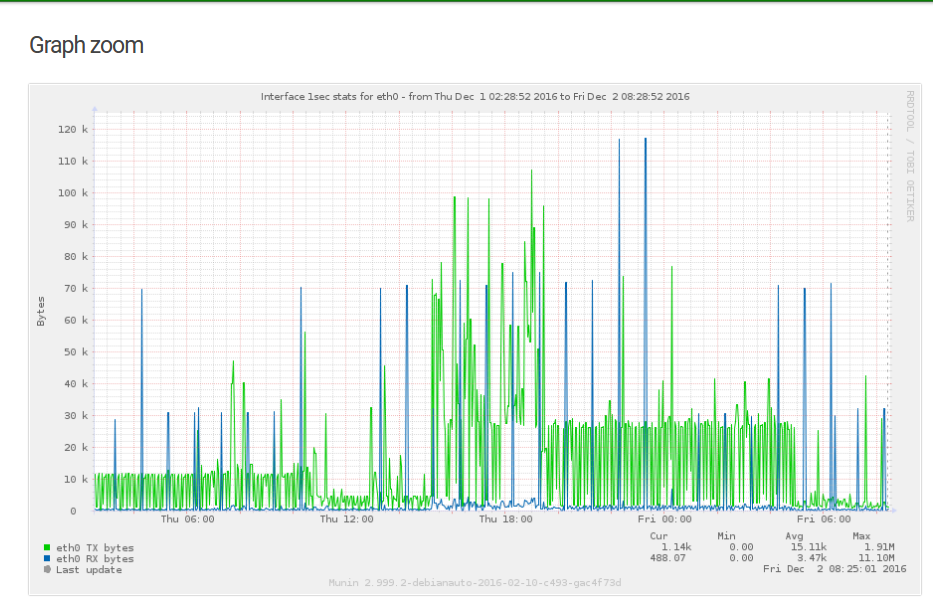
\includegraphics[scale=0.5]{imagenes/uso-red.png}  %el parámetro scale permite agrandar o achicar la imagen. En el nombre de archivo puede especificar directorios
	\caption{Monitorización de red.}
\end{figure}

Como podemos ver, el mayor uso de la red se encuentra en las horas de la tarde, sobre las 18:00 más o menos. Esto se debe a que son las horas del fin de la jornada de trabajo, y donde todos los empleados se conectan a la red para mandar correos, archivos, o el trabajo que hayan realizado. De ahí que estas horas el uso de red sea mucho más elevado que el resto.

Otro parámetro que vamos a ver será el uso de cpu.

\begin{figure}[H] %con el [H] le obligamos a situar aquí la figura
	\centering
	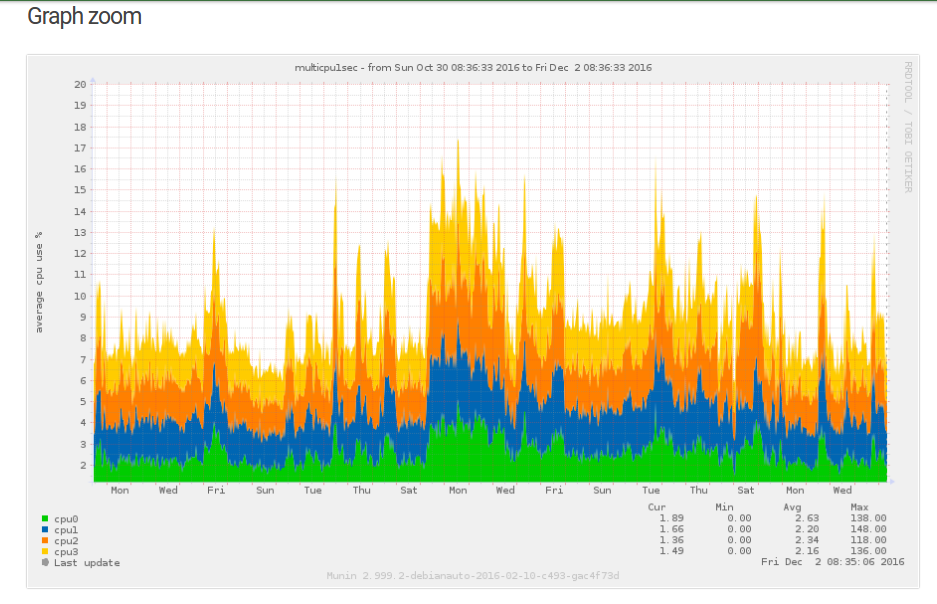
\includegraphics[scale=0.5]{imagenes/uso-cpu.png}  %el parámetro scale permite agrandar o achicar la imagen. En el nombre de archivo puede especificar directorios
	\caption{Monitorización de la cpu.}
\end{figure}

El uso de cpu lo vamos a monitorizar mensualmente, obteniendo el gráfico anterior.
En cuanto a los posibles comentarios de este gráfico, cabe destacar que los inicios y finales de las semanas como son domingos y lunes, el uso de cpu se dispara, por eso surgen los picos del gráfico, esto es podible que se deba a que durante el fin de semana, los empleados no hacen uso del servidor, pero las primeras horas de la semana y las últimas, estos necesitan conectarse y lo hacen casi todos a la vez(debido a que tengan un horario y se conectan al empezar y antes de finalizar la jornada), el resto de días el trabajo puede estar más repartido y los empleados no tienen la necesidad de conectarse y desconectarse casi todos a la vez.
Además se ve notablemente que hay una semana, en mitad del mes en la que el uso de la cpu es mayor que el resto de las semanas, ya que cuando esta acaba, disminuye bastante el uso de la cpu.

\section{Cuestión 7}

\subsection{\Large Escriba un breve resumen sobre alguno de los artículos donde se muestra el uso de strace o busque otro y coméntelo.}

El artículo que vamos a comentar va a ser el que se encuentra en la url de la referencia.\cite{strace}

Este artículo habla sobre la experiencia de un empleado con strace, al cual llamaron de una empresa para areglar un problema de un servidor el cual no permitia acceder a algunos archivos de la base de datos.

Después de esta pequeña experiecia nos habla de strace y de su uso.
Basándose en un ejemplo, nos explica el uso de esta herramienta, y de sus flags.
Una vez explicado su uso, pasa a hacer uso de strace sobre un ejemplo real, donde se da cuenta que el proceso que está siguiendo hace uso de TCP y del socket de UNIX.
Después de esto hace una comparación del proceso con el error y de el proceso sin el error, de tal forma que puede comparar entre ellos dónde está la mayor pérdida de tiempo.

Finalmente consigue ver que el error, que hace el proceso más lento estaba en un "log", y nos pone como ejemplo un código que usa la función sleep, y nos muestra cómo así podemos ver dónde está la función que gasta más tiempo, debido a que te muestra al final de cada sentencia el tiempo usado por esta.

\setlength{\parskip}{10pt}

Este artículo es bastante interesante, ya que nos explica el uso de strace, así como de algunas de las funcionalidades que presenta con sus flags, y además se presenta sobre un caso práctico y real, lo cual te motiva más a la hora de leerlo.

\section{Cuestión 8}

\subsection{\Large Escriba un script en Python o PHP y analice su comportamiento usando el profiler presentado.}

El Script que vamos a realizar va a ser un Script sencillo en el que imprimiremos por pantalla dos frases, y entre ellas vamos a poner un sleep de 2 segundos.

El sleep se lo vamos a añadir para ver los tiempos de cada función ya que las dos funciones de print tardarán en realizarse 0 segundos.

\begin{figure}[H] %con el [H] le obligamos a situar aquí la figura
	\centering
	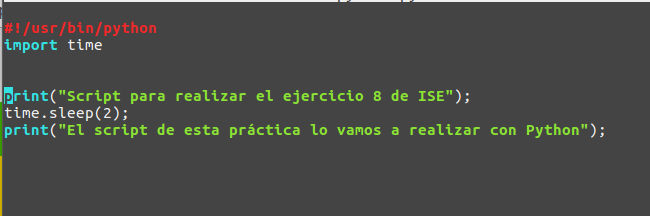
\includegraphics[scale=0.5]{imagenes/script-python.png}  %el parámetro scale permite agrandar o achicar la imagen. En el nombre de archivo puede especificar directorios
	\caption{Script para ejecutar el profiler sobre él.}
\end{figure}

Una vez hecho el script ejecutaremos sobre él el profiler, y en el caso de Python usaremos la función cProfile.

\begin{figure}[H] %con el [H] le obligamos a situar aquí la figura
	\centering
	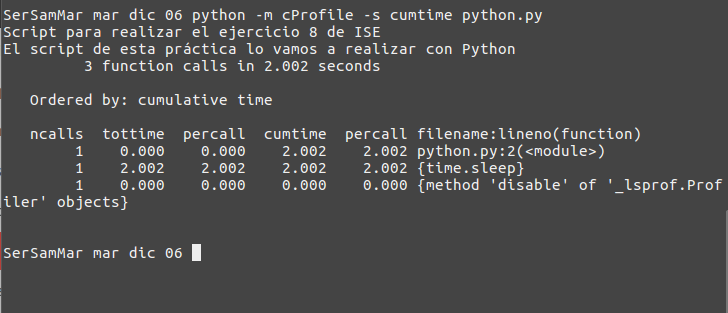
\includegraphics[scale=0.5]{imagenes/profiler-python.png}  %el parámetro scale permite agrandar o achicar la imagen. En el nombre de archivo puede especificar directorios
	\caption{Ejecución del profiler.}
\end{figure}

Como vemos, para ejecutar el script hacemos uso de cProfile, y además le he añadido cumTime para que vaya acumulando los tiempos de cada función.

Como vemos las dos funciones de print tardan 0 segundos, y entre ellas está la función sleep que es la que hace que el script tarde los 2 segundos en terminar de ejecutarse.

Para conocer el uso de la función cProfile he hecho uso de la página referenciada,\cite{profiler-python} en la que nos hace una introducción a los profilers de python.





\section{Cuestión 9}

\subsection{\Large Acceda a la consola mysql (o a través de phpMyAdmin) y muestre el resultado de mostrar el ”profile” de una consulta (la creación de la BD y la consulta la puede hacer libremente).}

Para acceder a mysql primero introducimos nuestra constraseña, lo cual indicamos con el flag -p, así nos pedirá la contraseña.

\begin{figure}[H] %con el [H] le obligamos a situar aquí la figura
	\centering
	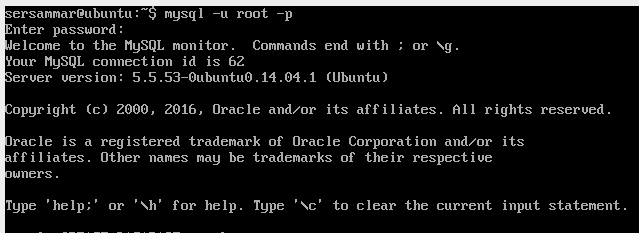
\includegraphics[scale=0.5]{imagenes/creacion-mysql.png}  %el parámetro scale permite agrandar o achicar la imagen. En el nombre de archivo puede especificar directorios
	\caption{Inicio de sedión de MySQL.}
\end{figure}

Una vez iniciada la sesión, lo que vamos a hacer es,lo primero activar el profiling, que por defecto está desactivado, para ello hacemos uso del comando SET PROFILING = 1;
\cite{mysql}

Una vez activado el profiling, haremos una serie de consultas sobre la base de datos, la primera será crear una base de datos, y después añadirle una tabla.Lo cual se muestra cómo hacerlo en la página que se cita a continuación, donde hay una pequeña introducción a SQL \cite{mysql-crea}

Por último, mostraremos los tiempos de cada sentencia haciendo uso del comando SHOW PROFILES; \cite{mysql2}


\begin{figure}[H] %con el [H] le obligamos a situar aquí la figura
	\centering
	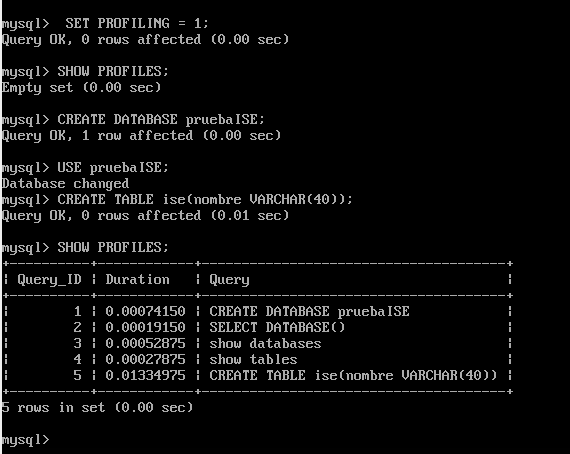
\includegraphics[scale=0.5]{imagenes/profiler-mysql.png}  %el parámetro scale permite agrandar o achicar la imagen. En el nombre de archivo puede especificar directorios
	\caption{Inicio de sedión de MySQL.}
\end{figure}

\newpage
%------------------------------------------------

\bibliography{citas} %archivo citas.bib que contiene las entradas 
\bibliographystyle{plain} % hay varias formas de citar

\end{document}
